\documentclass[tikz,border=8pt]{standalone}
% Shared pastel academic grammar for final-size technical-paper diagrams.
\usepackage[T1]{fontenc}
\usepackage{lmodern}
\usepackage{amsmath,amssymb}
\usepackage{xcolor}
\usepackage{tikz}
\usetikzlibrary{
  arrows.meta,
  backgrounds,
  calc,
  circuits.logic.US,
  decorations.pathreplacing,
  fit,
  matrix,
  patterns,
  positioning,
  shapes.geometric,
  shapes.symbols
}

\definecolor{ink}{RGB}{24,24,28}
\definecolor{midink}{RGB}{96,96,104}
\definecolor{paleink}{RGB}{184,184,190}
\definecolor{wash}{RGB}{241,240,237}
\definecolor{paper}{RGB}{255,255,253}
\definecolor{cyan}{RGB}{126,203,218}
\definecolor{cyanwash}{RGB}{211,238,242}
\definecolor{pink}{RGB}{235,139,158}
\definecolor{pinkwash}{RGB}{250,211,217}
\definecolor{purple}{RGB}{166,50,150}
\definecolor{purplewash}{RGB}{232,196,227}
\definecolor{gold}{RGB}{177,139,45}
\definecolor{goldwash}{RGB}{239,226,183}
\definecolor{slate}{RGB}{116,133,145}
\definecolor{slatewash}{RGB}{221,226,229}
\colorlet{muted}{midink}
\colorlet{rule}{paleink}
\colorlet{accent}{purple}
\colorlet{accentwash}{purplewash}
\colorlet{second}{cyan}
\colorlet{secondwash}{cyanwash}

\tikzset{
  every picture/.style={
    font=\rmfamily\footnotesize,
    text=ink,
    line cap=round,
    line join=round,
    >=Stealth
  },
  every node/.style={outer sep=0pt},
  panel mark/.style={font=\rmfamily\bfseries\footnotesize},
  primary/.style={font=\rmfamily\footnotesize},
  secondary/.style={font=\rmfamily\scriptsize,text=midink},
  signal name/.style={font=\ttfamily\footnotesize,anchor=east},
  scope trace/.style={draw=ink,line width=.62pt,line cap=butt,line join=miter},
  hairline/.style={draw=paleink,line width=.28pt,line cap=butt},
  dotted guide/.style={draw=midink,line width=.32pt,densely dotted},
  dashed scope/.style={draw=ink,line width=.45pt,dashed},
  transition/.style={-{Stealth[length=1.8mm,width=1.25mm]},draw=ink,line width=.58pt},
  transition label/.style={font=\rmfamily\scriptsize,fill=paper,inner sep=1.2pt},
  preedge/.style={circle,draw=ink,fill=paper,line width=.58pt,minimum size=8.2mm,inner sep=1pt},
  observed preedge/.style={preedge,fill=purplewash,double,double distance=1.15pt,line width=.62pt,minimum size=9.8mm},
  brace/.style={decorate,decoration={brace,mirror,amplitude=3pt},draw=ink,line width=.45pt},
  grid rule/.style={draw=slate,line width=.32pt,line cap=butt},
  outer rule/.style={draw=ink,line width=.82pt,line cap=butt,line join=miter},
  star mark/.style={star,star points=5,star point ratio=2.2,draw=ink,fill=purple,minimum size=5.1mm,inner sep=0pt},
  % Compatibility vocabulary used by the repository's other figures.
  flow/.style={-{Latex[length=4.5pt,width=3.2pt]},draw=ink,line width=.55pt},
  heavy flow/.style={-{Latex[length=5pt,width=3.6pt]},draw=ink,line width=.8pt},
  wire/.style={draw=ink,line width=.5pt},
  bus/.style={draw=ink,line width=1.05pt},
  guide/.style={draw=midink,line width=.4pt,dotted},
  alternate/.style={draw=ink,line width=.5pt,dashed},
  scope/.style={draw=ink,line width=.5pt,dashed,inner sep=6pt},
  block/.style={draw=ink,line width=.55pt,fill=paper,minimum height=8mm,inner xsep=5pt,inner ysep=4pt,align=center},
  operation/.style={block,fill=cyanwash,minimum width=17mm},
  register/.style={block,fill=paper,minimum width=16mm,minimum height=10mm},
  state/.style={circle,draw=ink,line width=.55pt,fill=cyanwash,minimum size=8mm,inner sep=1pt,align=center},
  terminal/.style={state,fill=purplewash,double,double distance=1.2pt,line width=.6pt},
  predicate/.style={diamond,aspect=1.8,draw=ink,line width=.55pt,fill=pinkwash,inner xsep=3pt,inner ysep=2pt,align=center},
  datum/.style={rectangle,draw=ink,line width=.5pt,fill=goldwash,minimum width=8mm,minimum height=6mm,inner sep=2pt,align=center},
  panel label/.style={font=\rmfamily\bfseries\footnotesize},
  local heading/.style={font=\rmfamily\bfseries\footnotesize},
  annotation/.style={font=\rmfamily\scriptsize,text=midink,align=center},
  heading/.style={font=\rmfamily\bfseries\small},
  subheading/.style={font=\rmfamily\bfseries\footnotesize},
  note/.style={font=\rmfamily\scriptsize,text=midink},
  label/.style={font=\rmfamily\bfseries\scriptsize},
  mono/.style={font=\ttfamily\footnotesize},
  tiny mono/.style={font=\ttfamily\scriptsize},
  count/.style={font=\rmfamily\bfseries\small},
  selected/.style={draw=ink,fill=purplewash,line width=.8pt},
  cell on/.style={fill=purple,draw=ink,line width=.3pt},
  cell off/.style={fill=paper,draw=paleink,line width=.3pt}
}

% Flat pastel facets and depth edges for restrained axonometric constructions.
\tikzset{
  cyan facet/.style={draw=ink,fill=cyanwash,line width=.5pt,line join=round},
  cyan side/.style={draw=ink,fill=cyan,line width=.5pt,line join=round},
  pink facet/.style={draw=ink,fill=pinkwash,line width=.5pt,line join=round},
  pink side/.style={draw=ink,fill=pink,line width=.5pt,line join=round},
  purple facet/.style={draw=ink,fill=purplewash,line width=.55pt,line join=round},
  purple side/.style={draw=ink,fill=purple,line width=.55pt,line join=round},
  gold facet/.style={draw=ink,fill=goldwash,line width=.5pt,line join=round},
  gold side/.style={draw=ink,fill=gold,line width=.5pt,line join=round},
  context facet/.style={draw=ink,fill=slatewash,line width=.45pt,line join=round},
  depth edge/.style={draw=midink,line width=.38pt},
  surface grid/.style={draw=slate,line width=.32pt},
  projection/.style={draw=midink,line width=.38pt,densely dashed},
  accent curve/.style={draw=purple,line width=1.05pt},
  cyan curve/.style={draw=cyan!70!ink,line width=.9pt},
  pink curve/.style={draw=pink!70!ink,line width=.9pt},
  gold curve/.style={draw=gold!80!ink,line width=.9pt}
}


\tikzset{
  local heading/.style={font=\rmfamily\bfseries\footnotesize},
  annotation/.style={secondary,align=center},
  wire/.style={scope trace,line width=.5pt},
  flow/.style={transition},
  heavy flow/.style={transition,line width=.82pt},
  rule/.style={hairline},
  cut top/.style={gold facet},
  cut side/.style={gold side},
  component/.style={
    circle,draw=ink,fill=paper,line width=.55pt,
    minimum size=3.1mm,inner sep=0pt
  },
  tree number/.style={font=\rmfamily\bfseries\footnotesize,align=center},
  tree note/.style={font=\rmfamily\scriptsize,text=midink,align=center},
  rail name/.style={font=\rmfamily\bfseries\footnotesize,anchor=west},
  file text/.style={font=\ttfamily\scriptsize,align=center}
}

\newcommand{\obliqueslab}[5]{%
  \path[#5 side]
    (#1,#2) -- ++(#3,0) -- ++(0,-.16) -- ++(-#3,0) -- cycle;
  \path[#5 facet]
    (#1,#2) -- ++(#3,0) -- ++(.55,.29) -- ++(-#3,0) -- cycle;
}

\newcommand{\thinplate}[5]{%
  \path[#5 side]
    (#1,#2) -- ++(#3,0) -- ++(0,-.10) -- ++(-#3,0) -- cycle;
  \path[#5 facet]
    (#1,#2) -- ++(#3,0) -- ++(.42,.22) -- ++(-#3,0) -- cycle;
}

\begin{document}
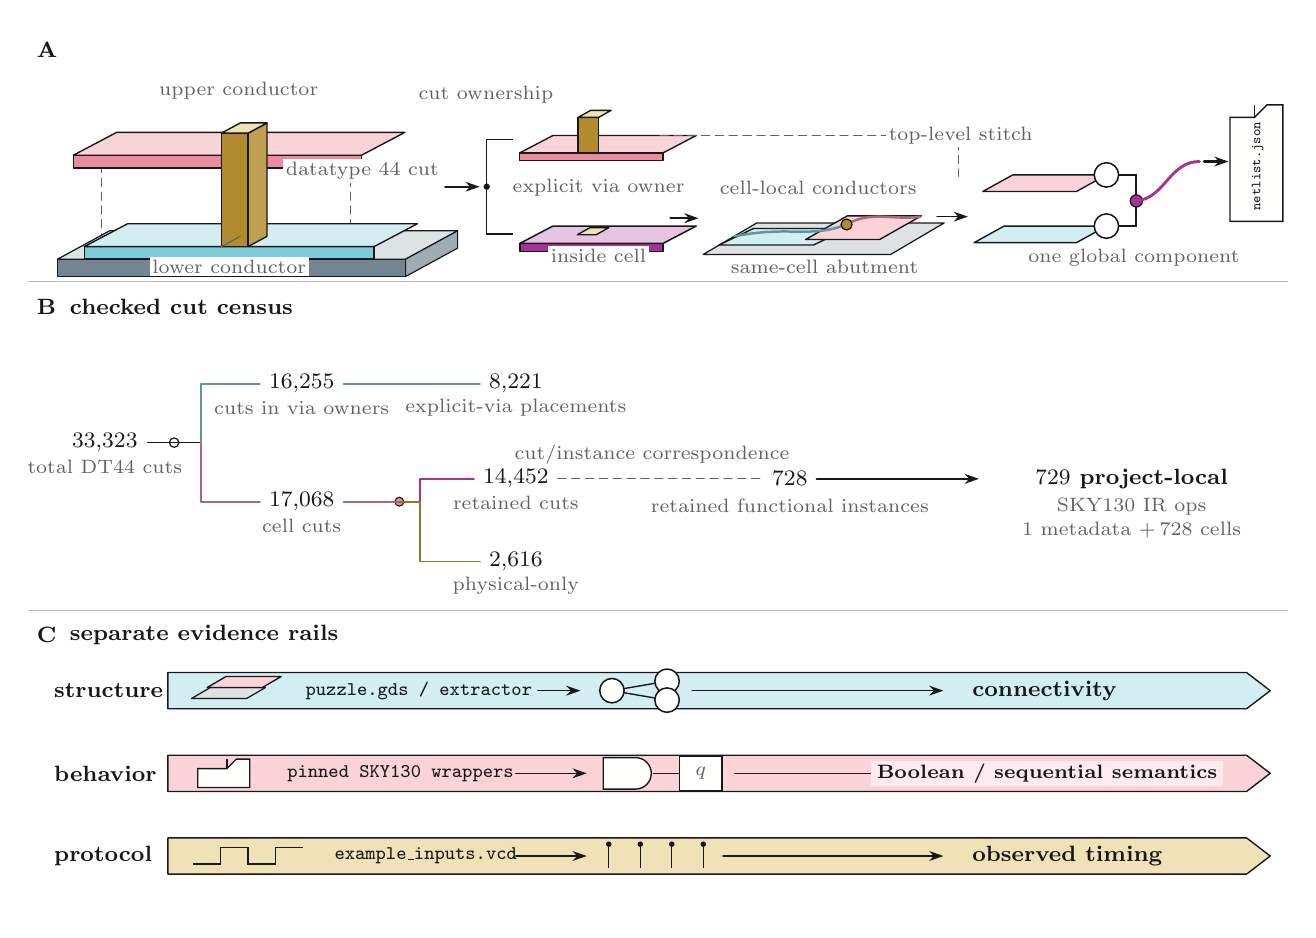
\begin{tikzpicture}[x=1cm,y=1cm]
  \path[use as bounding box] (0,0) rectangle (16,11.2);

  % A. Exploded geometry: conductor depth, DT44 ownership, and stitching.
  \node[panel mark,anchor=west] at (0,10.92) {A};

  % A coherent oblique scene: two conductor strata, a datatype-44 cut, and
  % the subsequent ownership/global-component interpretation.
  \draw[projection] (.94,8.48) -- (.94,9.72);
  \draw[projection] (4.10,8.48) -- (4.10,9.72);
  \path[context facet]
    (.38,8.26) -- (4.80,8.26) -- (5.46,8.62) -- (1.04,8.62) -- cycle;
  \path[fill=slate,draw=ink,line width=.42pt]
    (.38,8.26) -- (4.80,8.26) -- (4.80,8.04) -- (.38,8.04) -- cycle;
  \path[fill=slate!68,draw=ink,line width=.42pt]
    (4.80,8.26) -- (5.46,8.62) -- (5.46,8.40) -- (4.80,8.04) -- cycle;
  \draw[surface grid] (1.18,8.26) -- (1.84,8.62);
  \draw[surface grid] (3.68,8.26) -- (4.34,8.62);
  \obliqueslab{.72}{8.42}{3.68}{.50}{cyan}
  \node[annotation,anchor=south,fill=paper,inner sep=1pt] at (2.56,8.04)
    {lower conductor};

  \obliqueslab{.58}{9.58}{3.66}{.56}{pink}
  \node[annotation,anchor=south] at (2.68,10.17) {upper conductor};

  \path[cut side]
    (2.46,8.42) -- (2.80,8.42) -- (2.80,9.86) -- (2.46,9.86) -- cycle;
  \path[fill=gold!82,draw=ink,line width=.5pt]
    (2.80,8.42) -- (3.04,8.55) -- (3.04,9.99) -- (2.80,9.86) -- cycle;
  \path[cut top]
    (2.46,9.86) -- (2.80,9.86) -- (3.04,9.99) -- (2.70,9.99) -- cycle;
  \draw[depth edge] (2.46,8.42) -- (2.70,8.55);
  \node[annotation,anchor=west,fill=paper,inner sep=1.1pt] at (3.24,9.38)
    {datatype 44 cut};

  \draw[flow] (5.30,9.18) -- (5.74,9.18);
  \fill[ink] (5.83,9.18) circle (1.15pt);
  \draw[wire] (5.83,9.18) -- (5.83,9.78) -- (6.16,9.78);
  \draw[wire] (5.83,9.18) -- (5.83,8.58) -- (6.16,8.58);
  \node[annotation,anchor=south] at (5.82,10.12) {cut ownership};

  \thinplate{6.25}{9.61}{1.82}{.20}{pink}
  \path[cut side]
    (6.99,9.61) -- (7.25,9.61) -- (7.25,10.06) -- (6.99,10.06) -- cycle;
  \path[cut top]
    (6.99,10.06) -- (7.25,10.06) -- (7.41,10.15) -- (7.15,10.15) -- cycle;
  \node[annotation,anchor=north] at (7.25,9.39) {explicit via owner};

  \thinplate{6.25}{8.46}{1.82}{.20}{purple}
  \path[gold facet]
    (6.98,8.57) -- (7.22,8.57) -- (7.38,8.66) -- (7.14,8.66) -- cycle;
  \node[annotation,anchor=south,fill=paper,inner sep=1pt] at (7.25,8.18)
    {inside cell};

  \draw[flow] (8.16,8.78) -- (8.52,8.78);
  \path[context facet]
    (8.58,8.32) -- (10.96,8.32) -- (11.64,8.72) -- (9.26,8.72) -- cycle;
  \path[cyan facet]
    (8.78,8.44) -- (9.98,8.44) -- (10.42,8.65) -- (9.22,8.65) -- cycle;
  \path[pink facet]
    (9.88,8.51) -- (10.82,8.51) -- (11.35,8.81) -- (10.41,8.81) -- cycle;
  \draw[cyan curve] (8.98,8.55) .. controls (9.66,8.69) and (9.93,8.52) .. (10.40,8.70);
  \draw[pink curve] (10.40,8.70) .. controls (10.70,8.88) and (11.00,8.75) .. (11.34,8.80);
  \filldraw[draw=ink,fill=gold,line width=.45pt] (10.40,8.70) circle (2.0pt);
  \node[annotation,anchor=south] at (10.04,8.96) {cell-local conductors};
  \node[annotation,anchor=south,fill=paper,inner sep=1pt] at (10.12,8.04)
    {same-cell abutment};

  \draw[projection] (8.03,9.83) -- (11.82,9.83) -- (11.82,9.31);
  \node[annotation,fill=paper,inner sep=1.2pt] at (11.85,9.83)
    {top-level stitch};
  \draw[flow] (11.55,8.80) -- (11.94,8.80);
  \path[cyan facet]
    (12.02,8.47) -- (13.32,8.47) -- (13.70,8.68) -- (12.40,8.68) -- cycle;
  \path[pink facet]
    (12.13,9.12) -- (13.32,9.12) -- (13.70,9.33) -- (12.51,9.33) -- cycle;
  \node[component] (lowerPin) at (13.70,8.68) {};
  \node[component] (upperPin) at (13.70,9.33) {};
  \draw[outer rule] (lowerPin) -- (14.08,8.68) -- (14.08,9.33) -- (upperPin);
  \filldraw[draw=ink,fill=purple,line width=.45pt] (14.08,9.00) circle (2.2pt);
  \draw[accent curve] (14.08,9.00) .. controls (14.44,9.03) and (14.50,9.50) .. (14.88,9.50);
  \node[annotation,anchor=north] at (14.05,8.50) {one global component};
  \draw[heavy flow] (14.94,9.50) -- (15.25,9.50);
  \draw[wire,fill=paper]
    (15.27,8.74) -- (15.94,8.74) -- (15.94,10.22) --
    (15.74,10.22) -- (15.58,10.06) -- (15.27,10.06) -- cycle;
  \draw[wire] (15.58,10.06) -- (15.58,10.22);
  \node[font=\ttfamily\tiny,rotate=90,align=center] at (15.62,9.44)
    {netlist.json};

  \draw[rule,line width=.45pt] (0,7.98) -- (16,7.98);

  % B. Exact checked census, shown as a split tree rather than a sequence.
  \node[panel mark,anchor=west] at (0,7.66) {B};
  \node[local heading,anchor=west] at (.42,7.66) {checked cut census};

  \node[tree number] (total) at (.98,5.93) {$33{,}323$};
  \node[tree note] at (.98,5.62) {total DT44 cuts};
  \filldraw[draw=ink,fill=paper,line width=.45pt] (1.86,5.93) circle (1.7pt);

  \node[tree number] (viaCuts) at (3.48,6.68) {$16{,}255$};
  \node[tree note] at (3.48,6.37) {cuts in via owners};
  \node[tree number] (cellCuts) at (3.48,5.18) {$17{,}068$};
  \node[tree note] at (3.48,4.87) {cell cuts};
  \draw[wire] (total.east) -- (1.86,5.93);
  \draw[wire] (1.86,5.93) -- (2.20,5.93);
  \draw[cyan curve,line width=.7pt] (2.20,5.93) -- (2.20,6.68) -- (viaCuts.west);
  \draw[pink curve,line width=.7pt] (2.20,5.93) -- (2.20,5.18) -- (cellCuts.west);

  \node[tree number] (viaOwners) at (6.20,6.68) {$8{,}221$};
  \node[tree note] at (6.20,6.37) {explicit-via placements};
  \draw[cyan curve,line width=.7pt] (viaCuts.east) -- (viaOwners.west);

  \node[tree number] (retainedCuts) at (6.20,5.47) {$14{,}452$};
  \node[tree note] at (6.20,5.16) {retained cuts};
  \node[tree number] (physicalCuts) at (6.20,4.42) {$2{,}616$};
  \node[tree note] at (6.20,4.11) {physical-only};
  \filldraw[draw=ink,fill=pink,line width=.4pt] (4.72,5.18) circle (1.6pt);
  \draw[pink curve,line width=.7pt] (cellCuts.east) -- (4.72,5.18);
  \draw[draw=purple,line width=.7pt] (4.72,5.18) -- (4.98,5.18) -- (4.98,5.47) -- (retainedCuts.west);
  \draw[gold curve,line width=.7pt] (4.72,5.18) -- (4.98,5.18) -- (4.98,4.42) -- (physicalCuts.west);

  \node[tree number] (instances) at (9.68,5.47) {$728$};
  \node[tree note] at (9.68,5.13) {retained functional instances};
  \draw[projection] (retainedCuts.east) -- (instances.west);
  \node[annotation,fill=paper,inner sep=1pt] at (7.93,5.78)
    {cut/instance correspondence};

  \node[tree number] (ops) at (14.02,5.47) {$729$ project-local};
  \node[tree note] at (14.02,5.12) {SKY130 IR ops};
  \node[tree note] at (14.02,4.82) {$1$ metadata $+\,728$ cells};
  \draw[heavy flow] (instances.east) -- (12.08,5.47);

  \draw[rule,line width=.45pt] (0,3.80) -- (16,3.80);

  % C. Independent evidence rails prevent a geometry-to-behavior shortcut.
  \node[panel mark,anchor=west] at (0,3.49) {C};
  \node[local heading,anchor=west] at (.42,3.49) {separate evidence rails};

  \path[cyan facet]
    (1.78,2.55) -- (15.48,2.55) -- (15.78,2.78) -- (15.48,3.01) --
    (1.78,3.01) -- cycle;
  \node[rail name] at (.22,2.78) {structure};
  \path[context facet]
    (2.08,2.68) -- (2.78,2.68) -- (3.02,2.82) -- (2.32,2.82) -- cycle;
  \path[pink facet]
    (2.28,2.82) -- (2.98,2.82) -- (3.22,2.96) -- (2.52,2.96) -- cycle;
  \node[file text,anchor=west,fill=cyanwash,inner xsep=2pt,inner ysep=1pt]
    at (3.46,2.78) {puzzle.gds / extractor};
  \draw[flow] (6.48,2.78) -- (7.02,2.78);
  \node[component] (sn0) at (7.42,2.78) {};
  \node[component] (sn1) at (8.12,2.90) {};
  \node[component] (sn2) at (8.12,2.66) {};
  \draw[wire] (sn0) -- (sn1);
  \draw[wire] (sn0) -- (sn2);
  \draw[flow] (8.44,2.78) -- (11.63,2.78);
  \node[local heading,anchor=west] at (11.88,2.78) {connectivity};

  \path[pink facet]
    (1.78,1.50) -- (15.48,1.50) -- (15.78,1.73) -- (15.48,1.96) --
    (1.78,1.96) -- cycle;
  \node[rail name] at (.22,1.73) {behavior};
  \draw[wire,fill=paper]
    (2.16,1.55) -- (2.82,1.55) -- (2.82,1.91) --
    (2.65,1.91) -- (2.53,1.79) -- (2.16,1.79) -- cycle;
  \draw[wire] (2.53,1.79) -- (2.53,1.91);
  \node[file text,anchor=west] at (3.18,1.73) {pinned SKY130 wrappers};
  \draw[flow] (6.20,1.73) -- (7.10,1.73);
  \draw[wire,fill=paper]
    (7.31,1.53) -- (7.31,1.93) -- (7.72,1.93)
    arc[start angle=90,end angle=-90,radius=.20] -- cycle;
  \draw[wire] (7.94,1.73) -- (8.28,1.73);
  \draw[wire,fill=paper] (8.28,1.51) rectangle (8.82,1.95);
  \node[annotation] at (8.55,1.73) {$q$};
  \draw[flow] (8.98,1.73) -- (11.63,1.73);
  \node[font=\rmfamily\bfseries\scriptsize,anchor=east,fill=pink!18,inner xsep=2pt,inner ysep=1pt] at (15.18,1.73)
    {Boolean / sequential semantics};

  \path[gold facet]
    (1.78,.45) -- (15.48,.45) -- (15.78,.68) -- (15.48,.91) --
    (1.78,.91) -- cycle;
  \node[rail name] at (.22,.68) {protocol};
  \draw[wire]
    (2.10,.58) -- (2.45,.58) -- (2.45,.79) -- (2.80,.79) --
    (2.80,.58) -- (3.15,.58) -- (3.15,.79) -- (3.50,.79);
  \node[file text,anchor=west] at (3.78,.68) {example\_inputs.vcd};
  \draw[flow] (6.20,.68) -- (7.10,.68);
  \foreach \x in {7.38,7.78,8.18,8.58}{
    \draw[wire] (\x,.53) -- (\x,.83);
    \fill[ink] (\x,.83) circle (1pt);
  }
  \draw[flow] (8.83,.68) -- (11.63,.68);
  \node[local heading,anchor=west] at (11.88,.68) {observed timing};
\end{tikzpicture}
\end{document}
